\begin{figure}[H]\centering
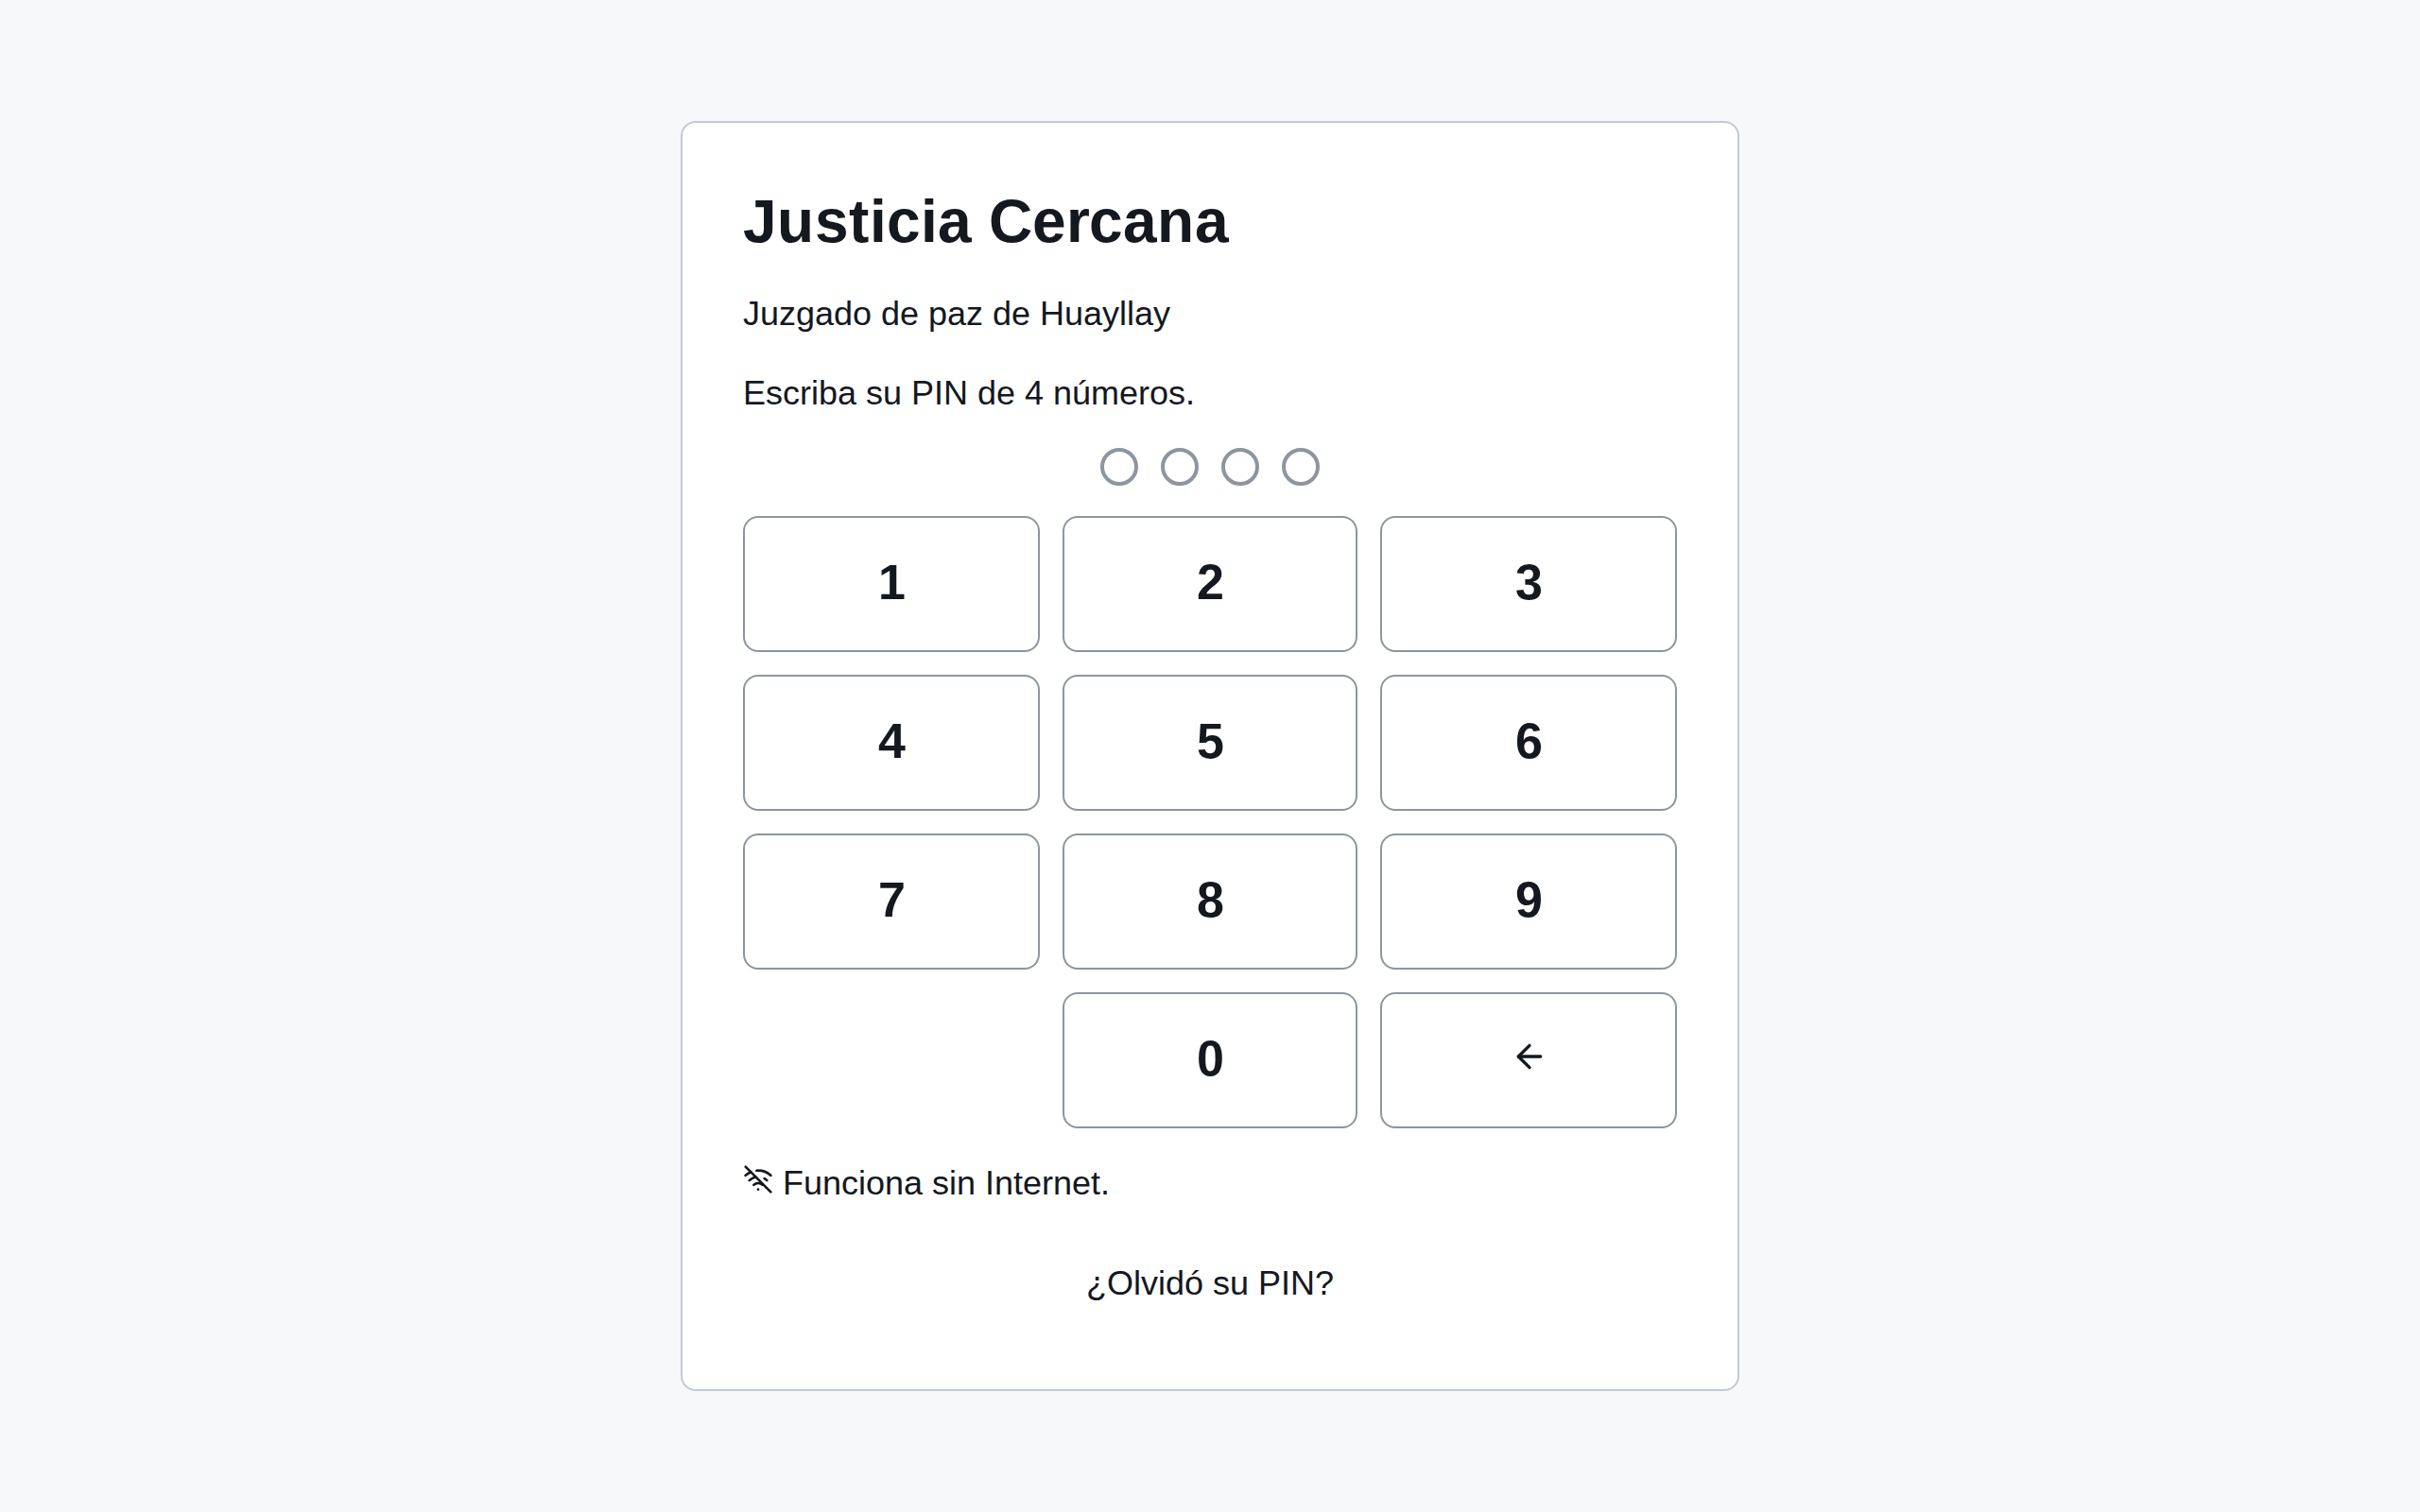
\includegraphics[width=0.86\linewidth]{capturas/P-00_ingreso-pin.png}
\caption{P-00 · Ingreso. PIN numérico de 4 dígitos con teclado grande, funciona sin Internet}
\end{figure}
\begin{figure}[H]\centering
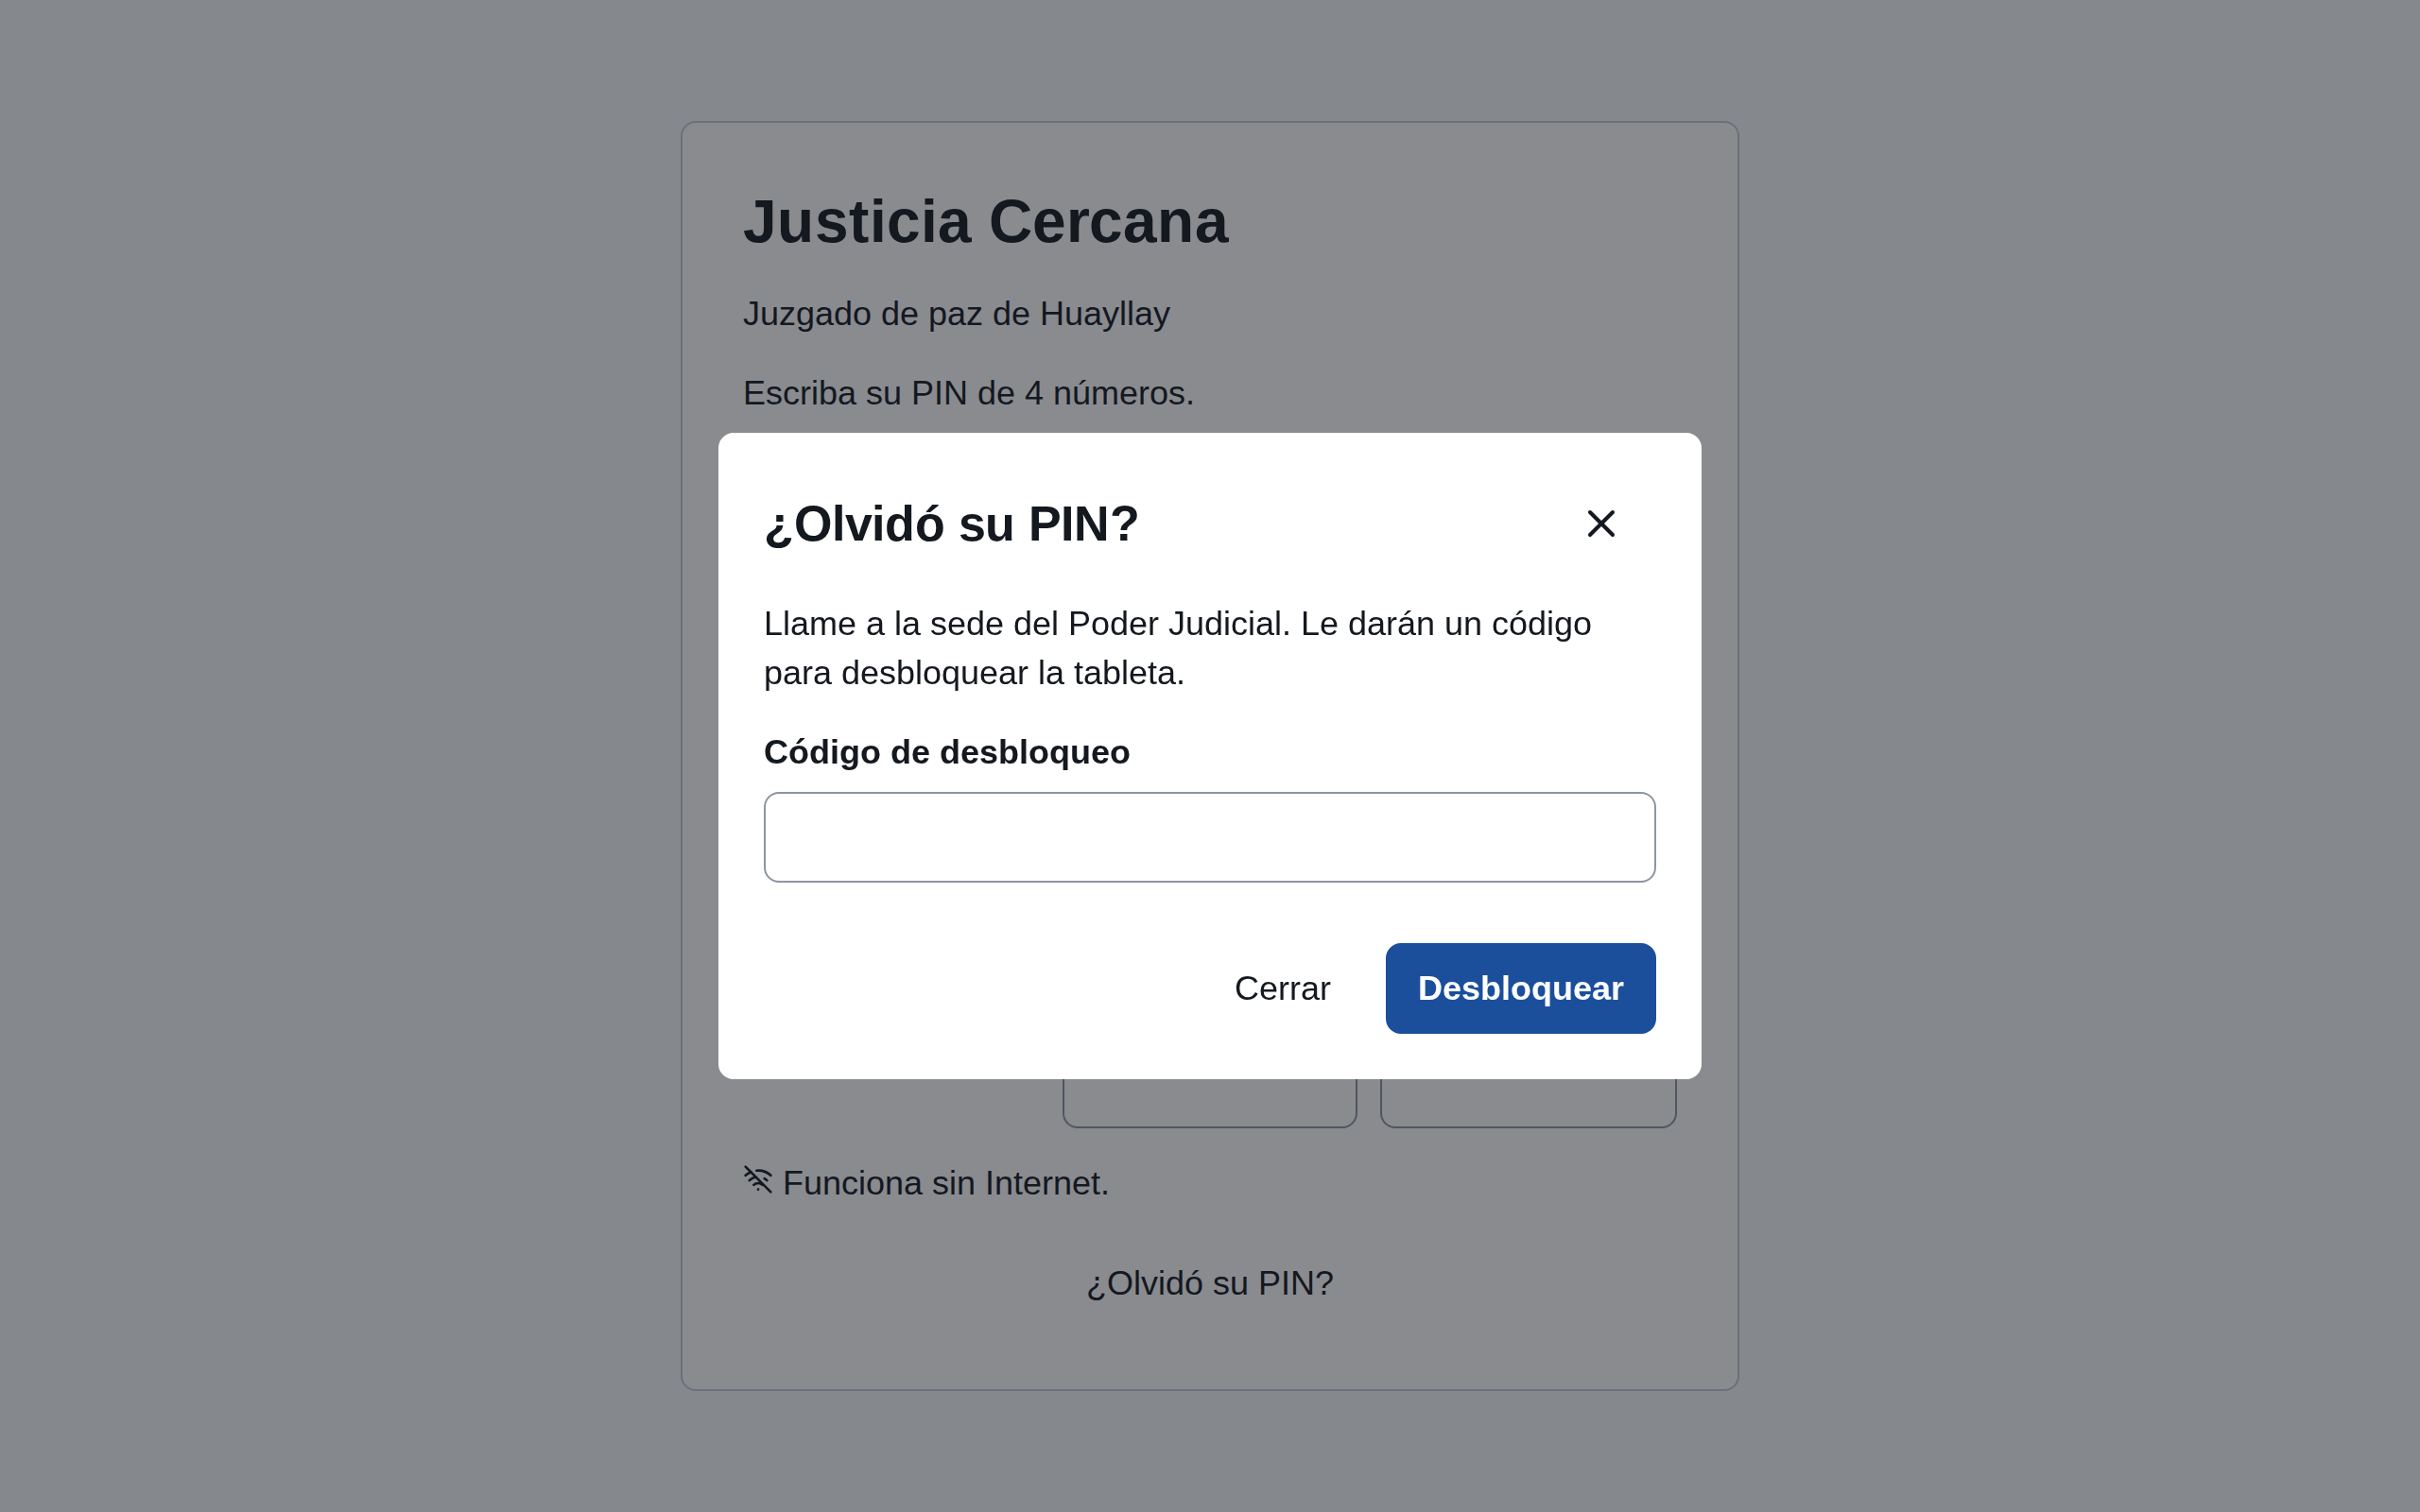
\includegraphics[width=0.86\linewidth]{capturas/P-00b_olvido-pin.png}
\caption{P-00 · Olvidó el PIN. Recuperación explicada en lenguaje cotidiano, sin bloqueo del trabajo}
\end{figure}
\begin{figure}[H]\centering
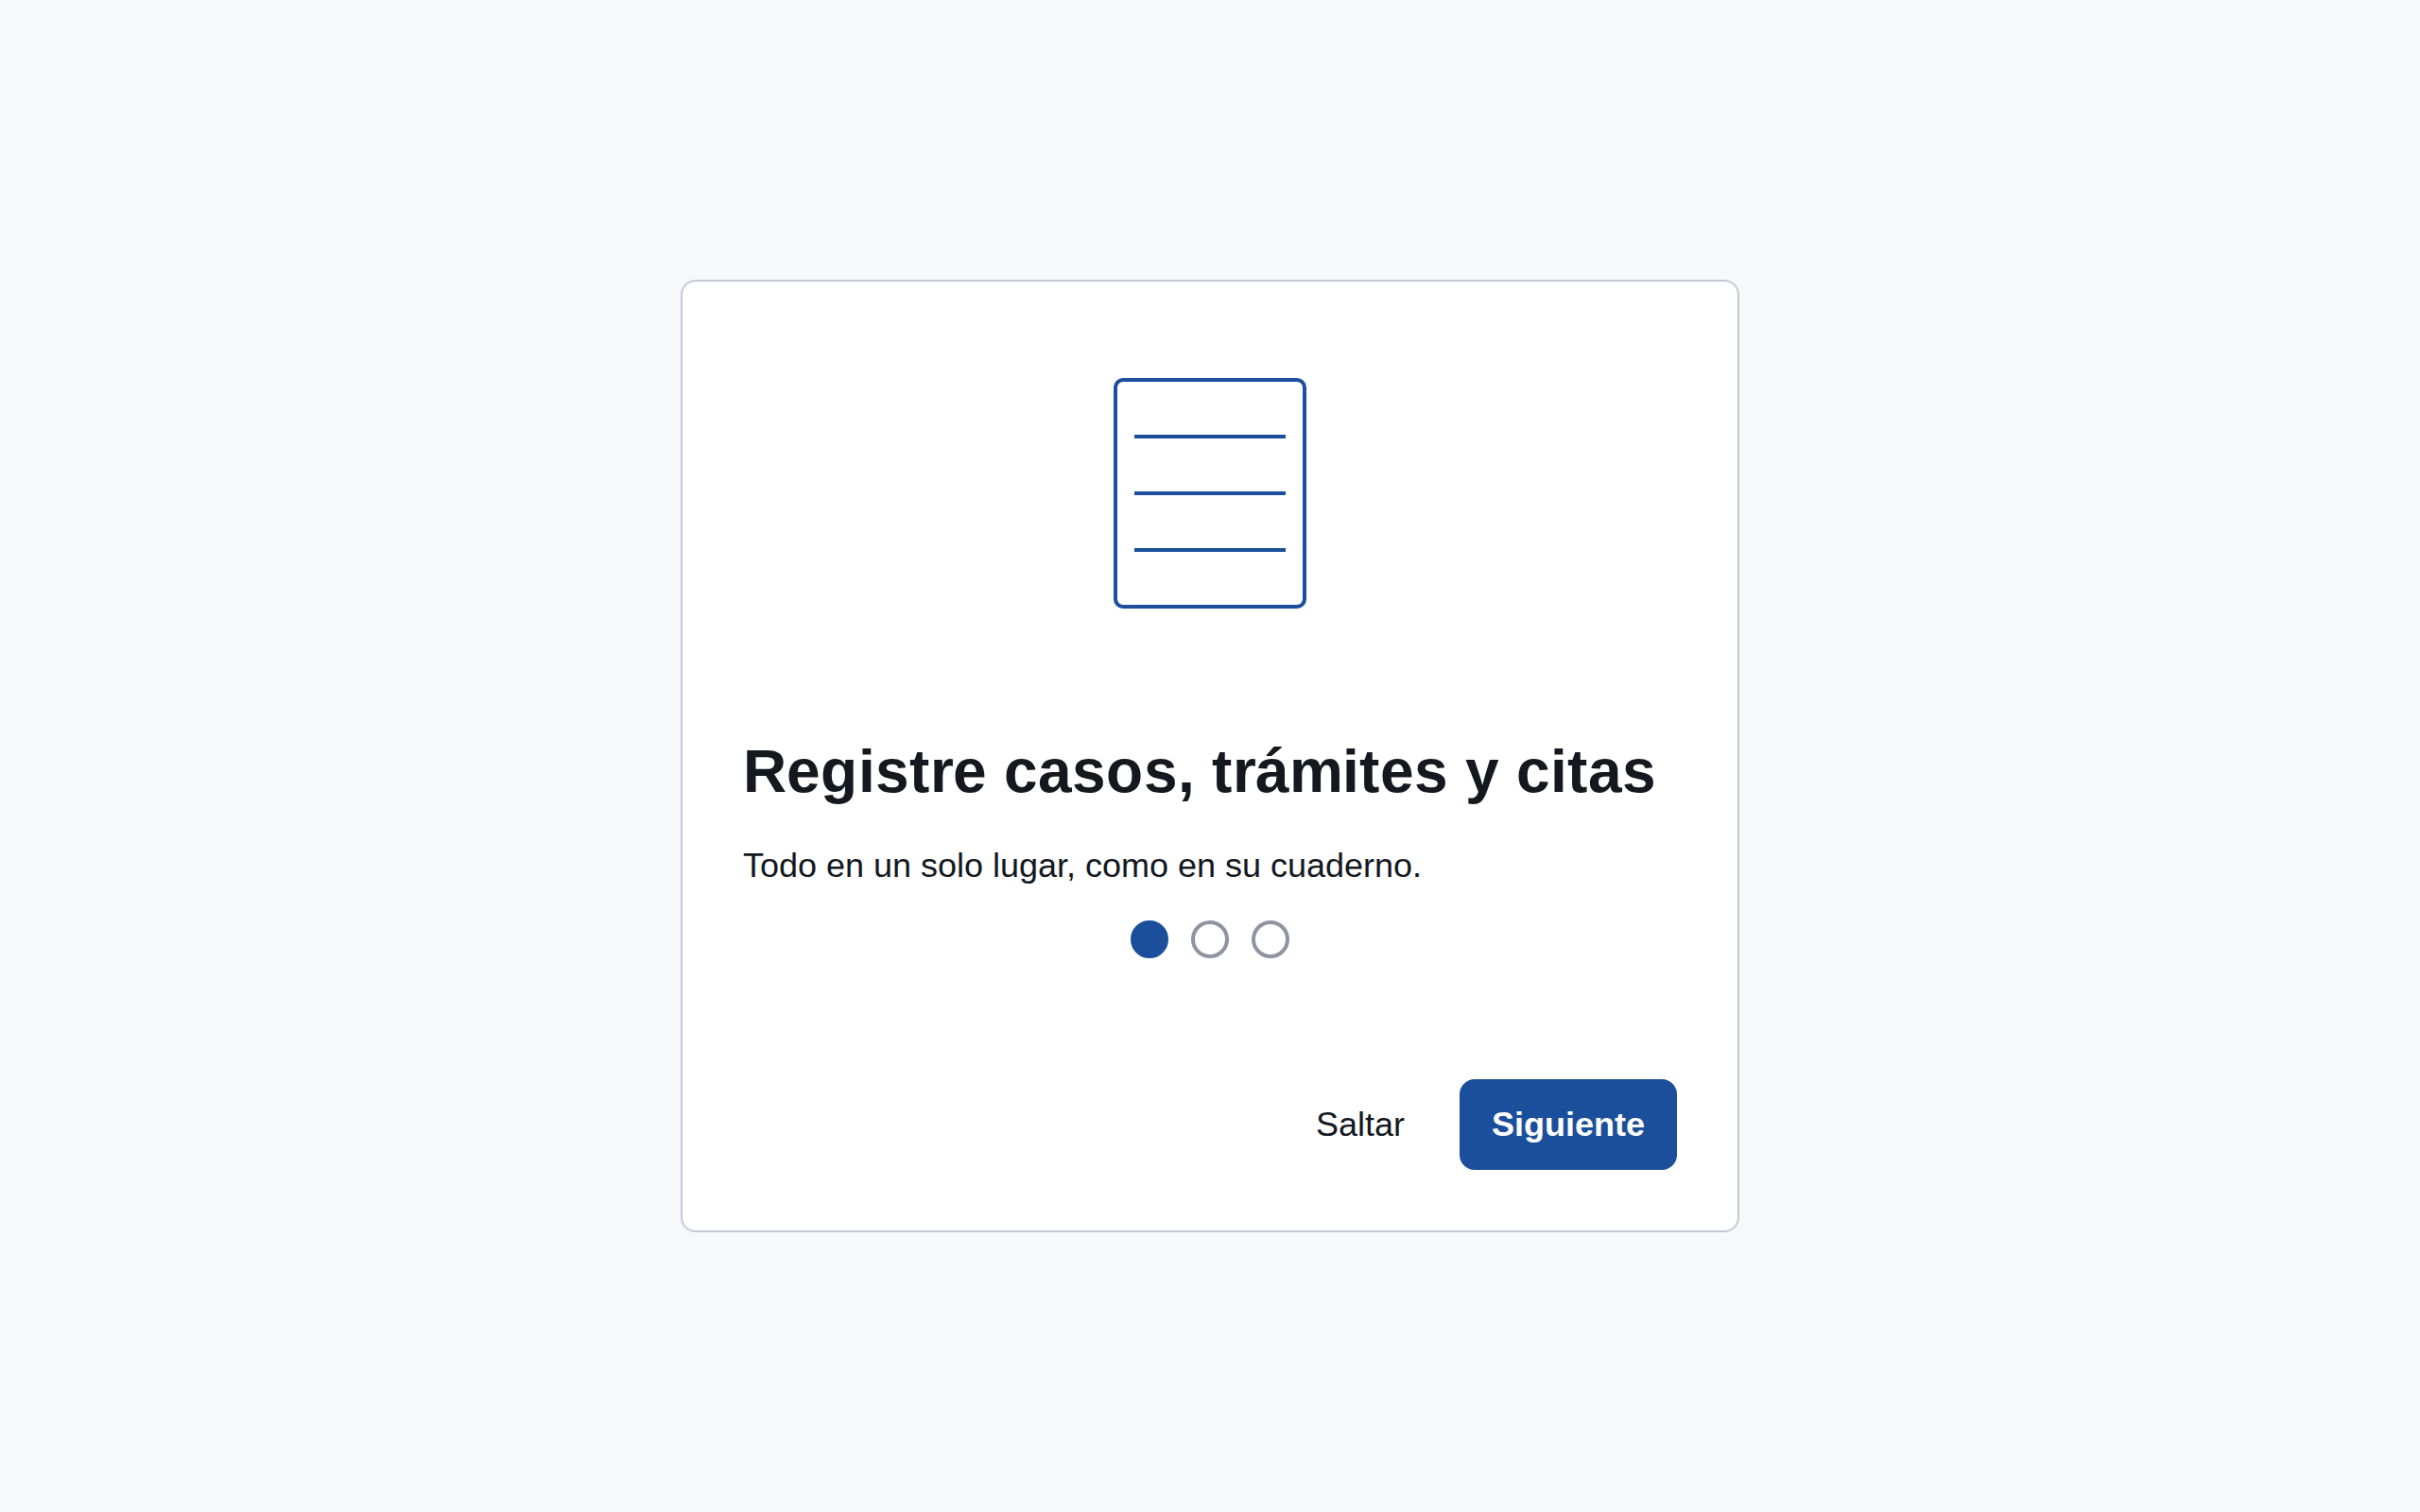
\includegraphics[width=0.86\linewidth]{capturas/P-00c_intro-1.png}
\caption{P-00b · Introducción 1 de 3. Introducción de tres pantallas con botón Saltar visible}
\end{figure}
\begin{figure}[H]\centering
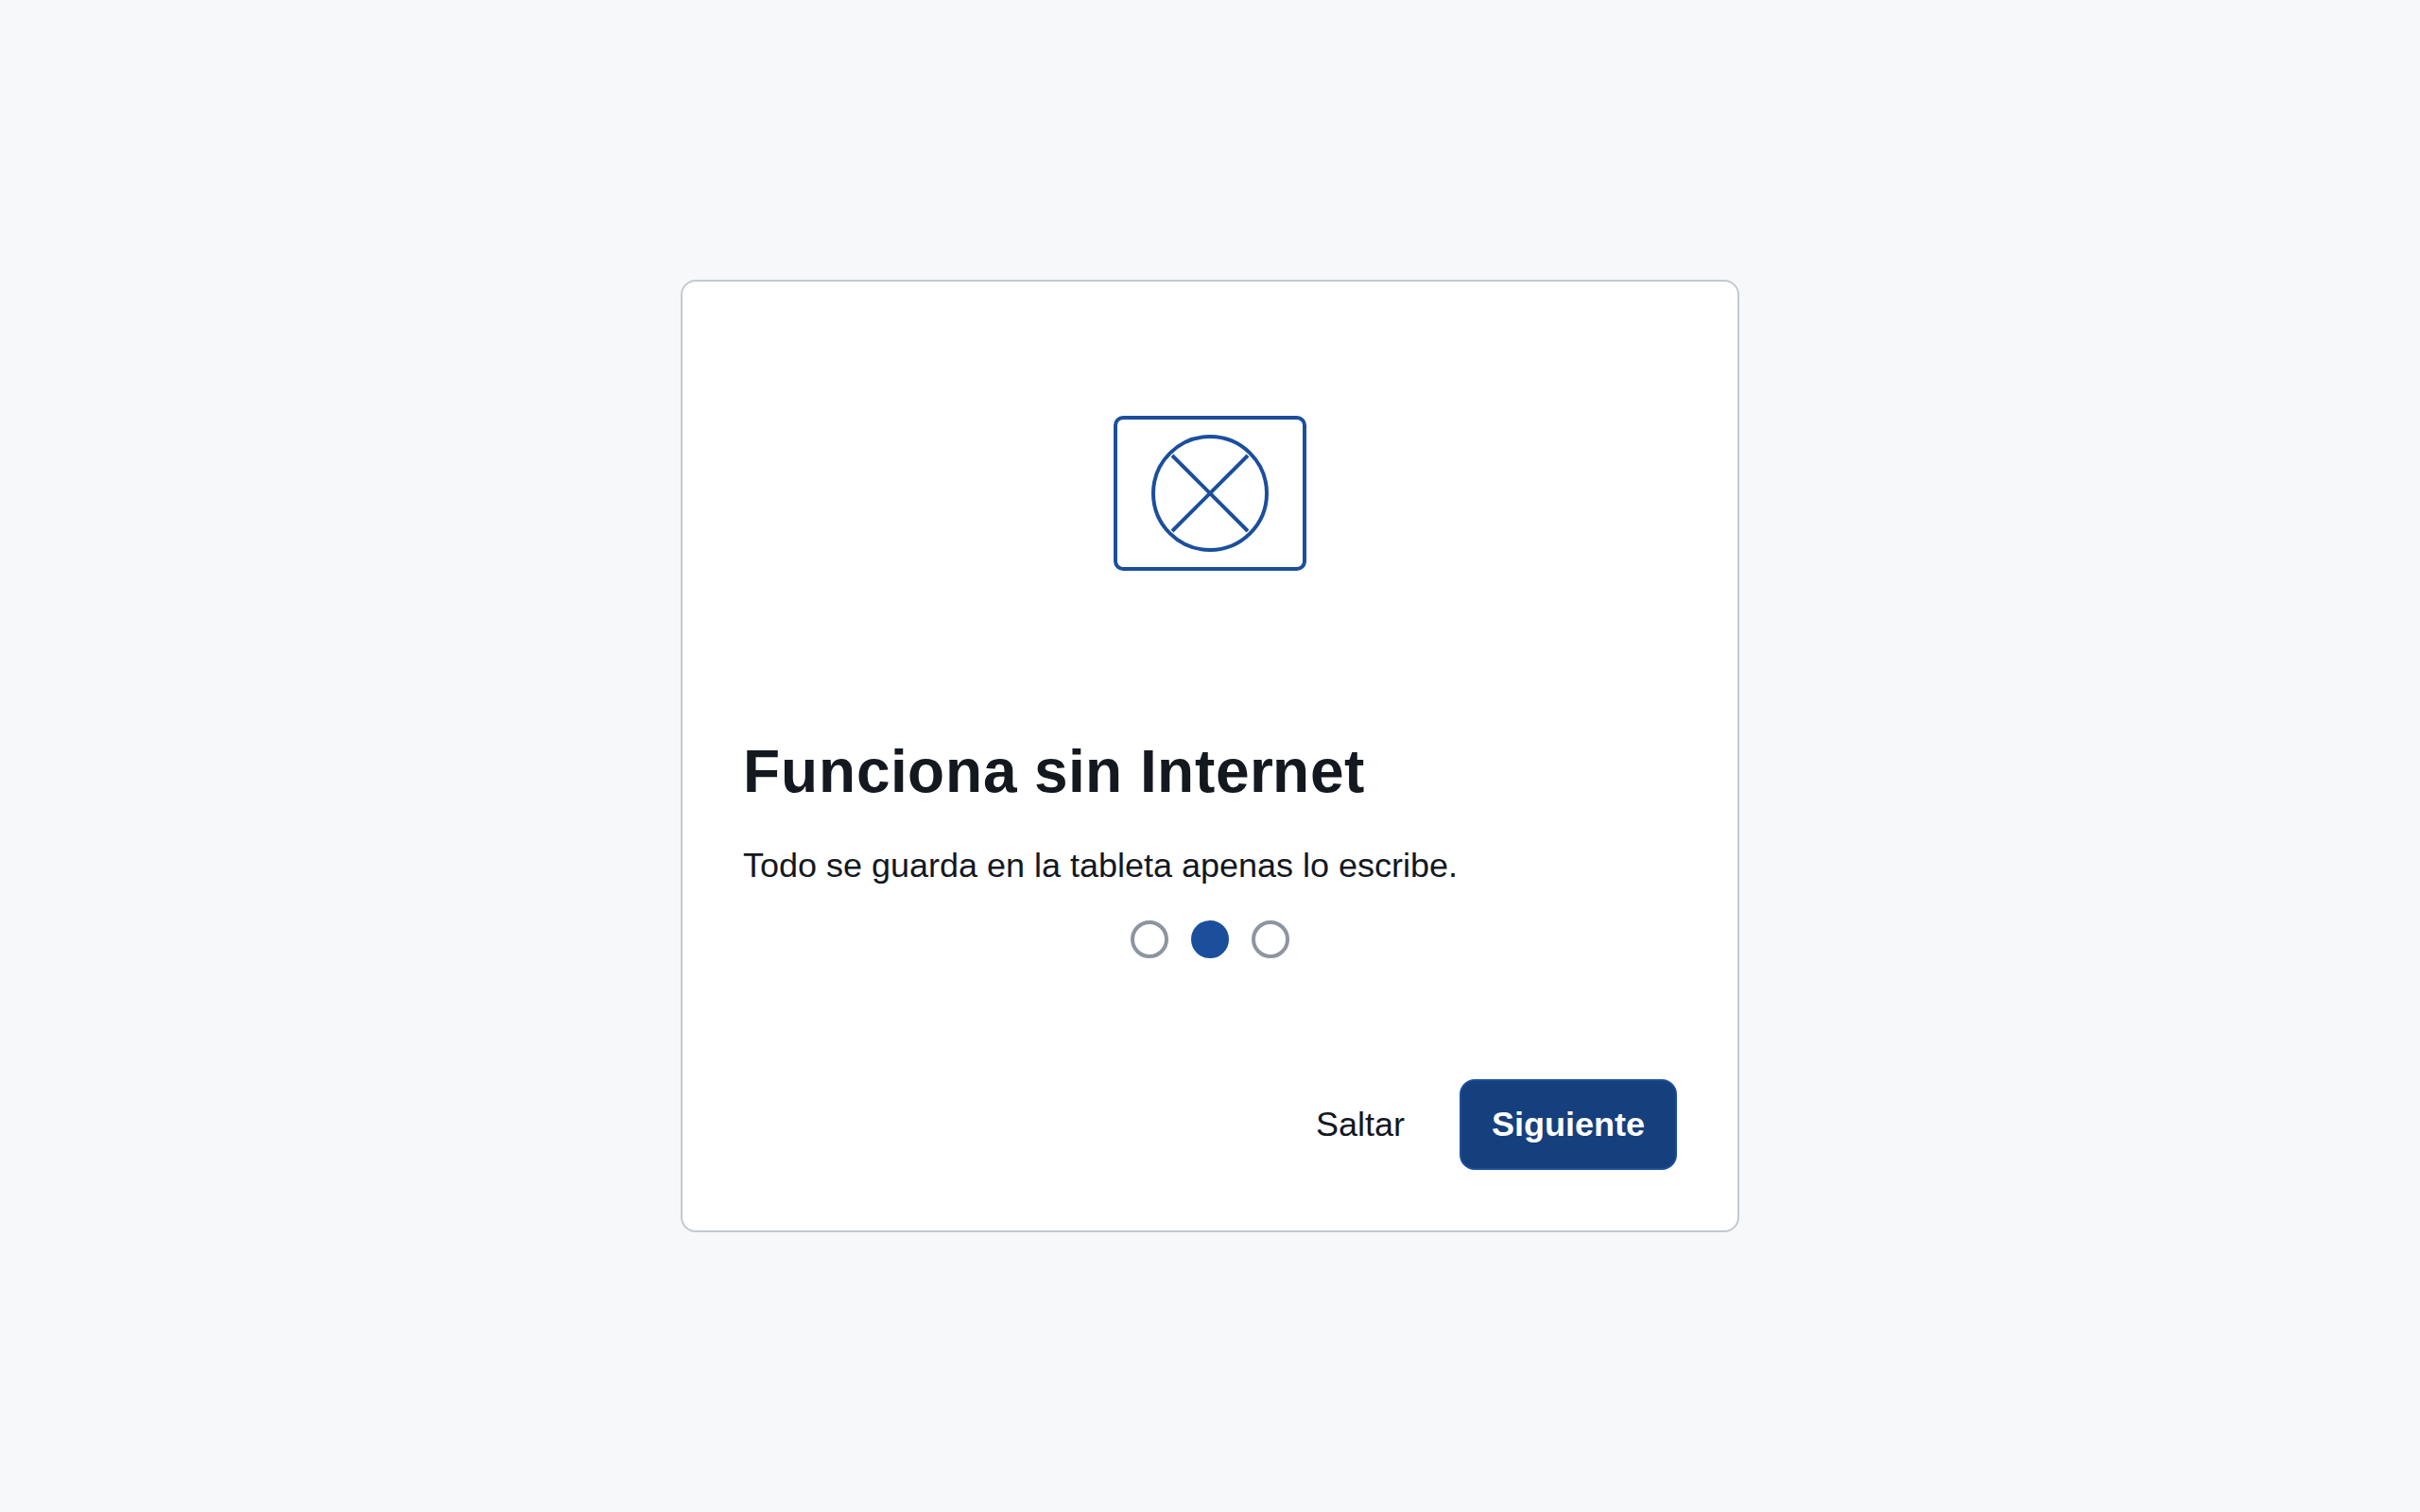
\includegraphics[width=0.86\linewidth]{capturas/P-00d_intro-2.png}
\caption{P-00b · Introducción 2 de 3. Se explica el trabajo sin Internet antes de usar la aplicación}
\end{figure}
\begin{figure}[H]\centering
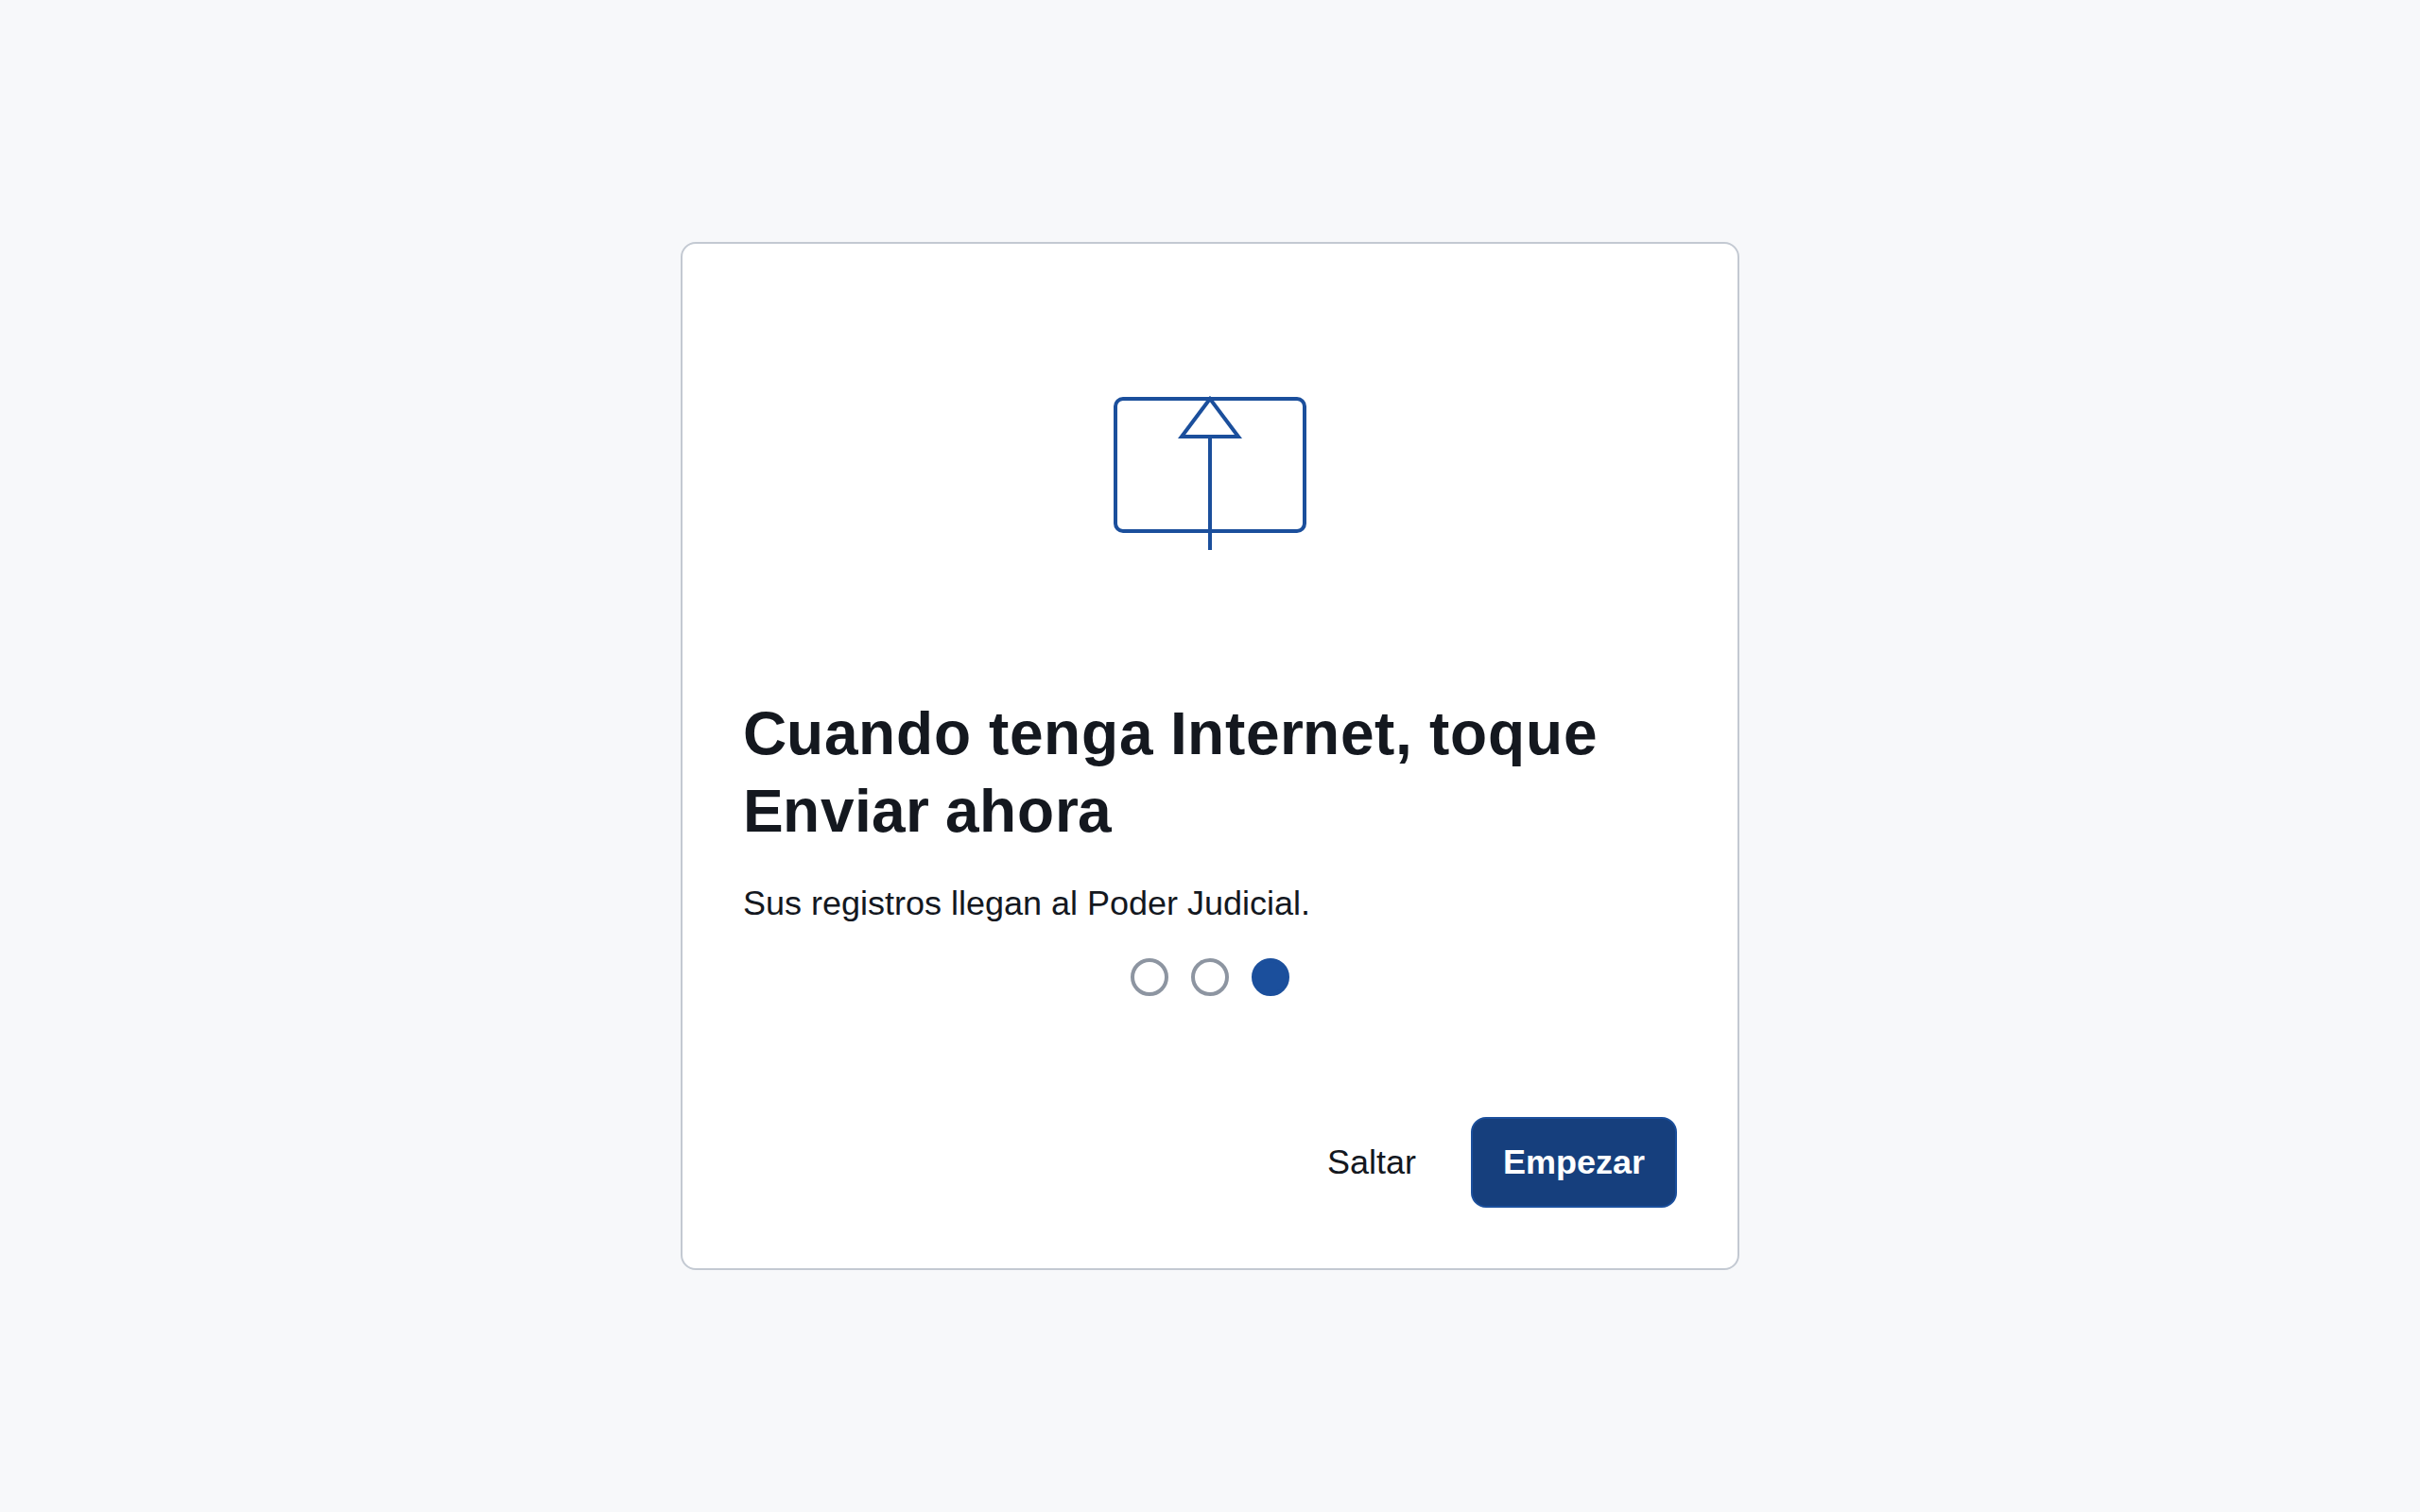
\includegraphics[width=0.86\linewidth]{capturas/P-00e_intro-3.png}
\caption{P-00b · Introducción 3 de 3. Se enseña el botón Enviar ahora antes de necesitarlo}
\end{figure}
\begin{figure}[H]\centering
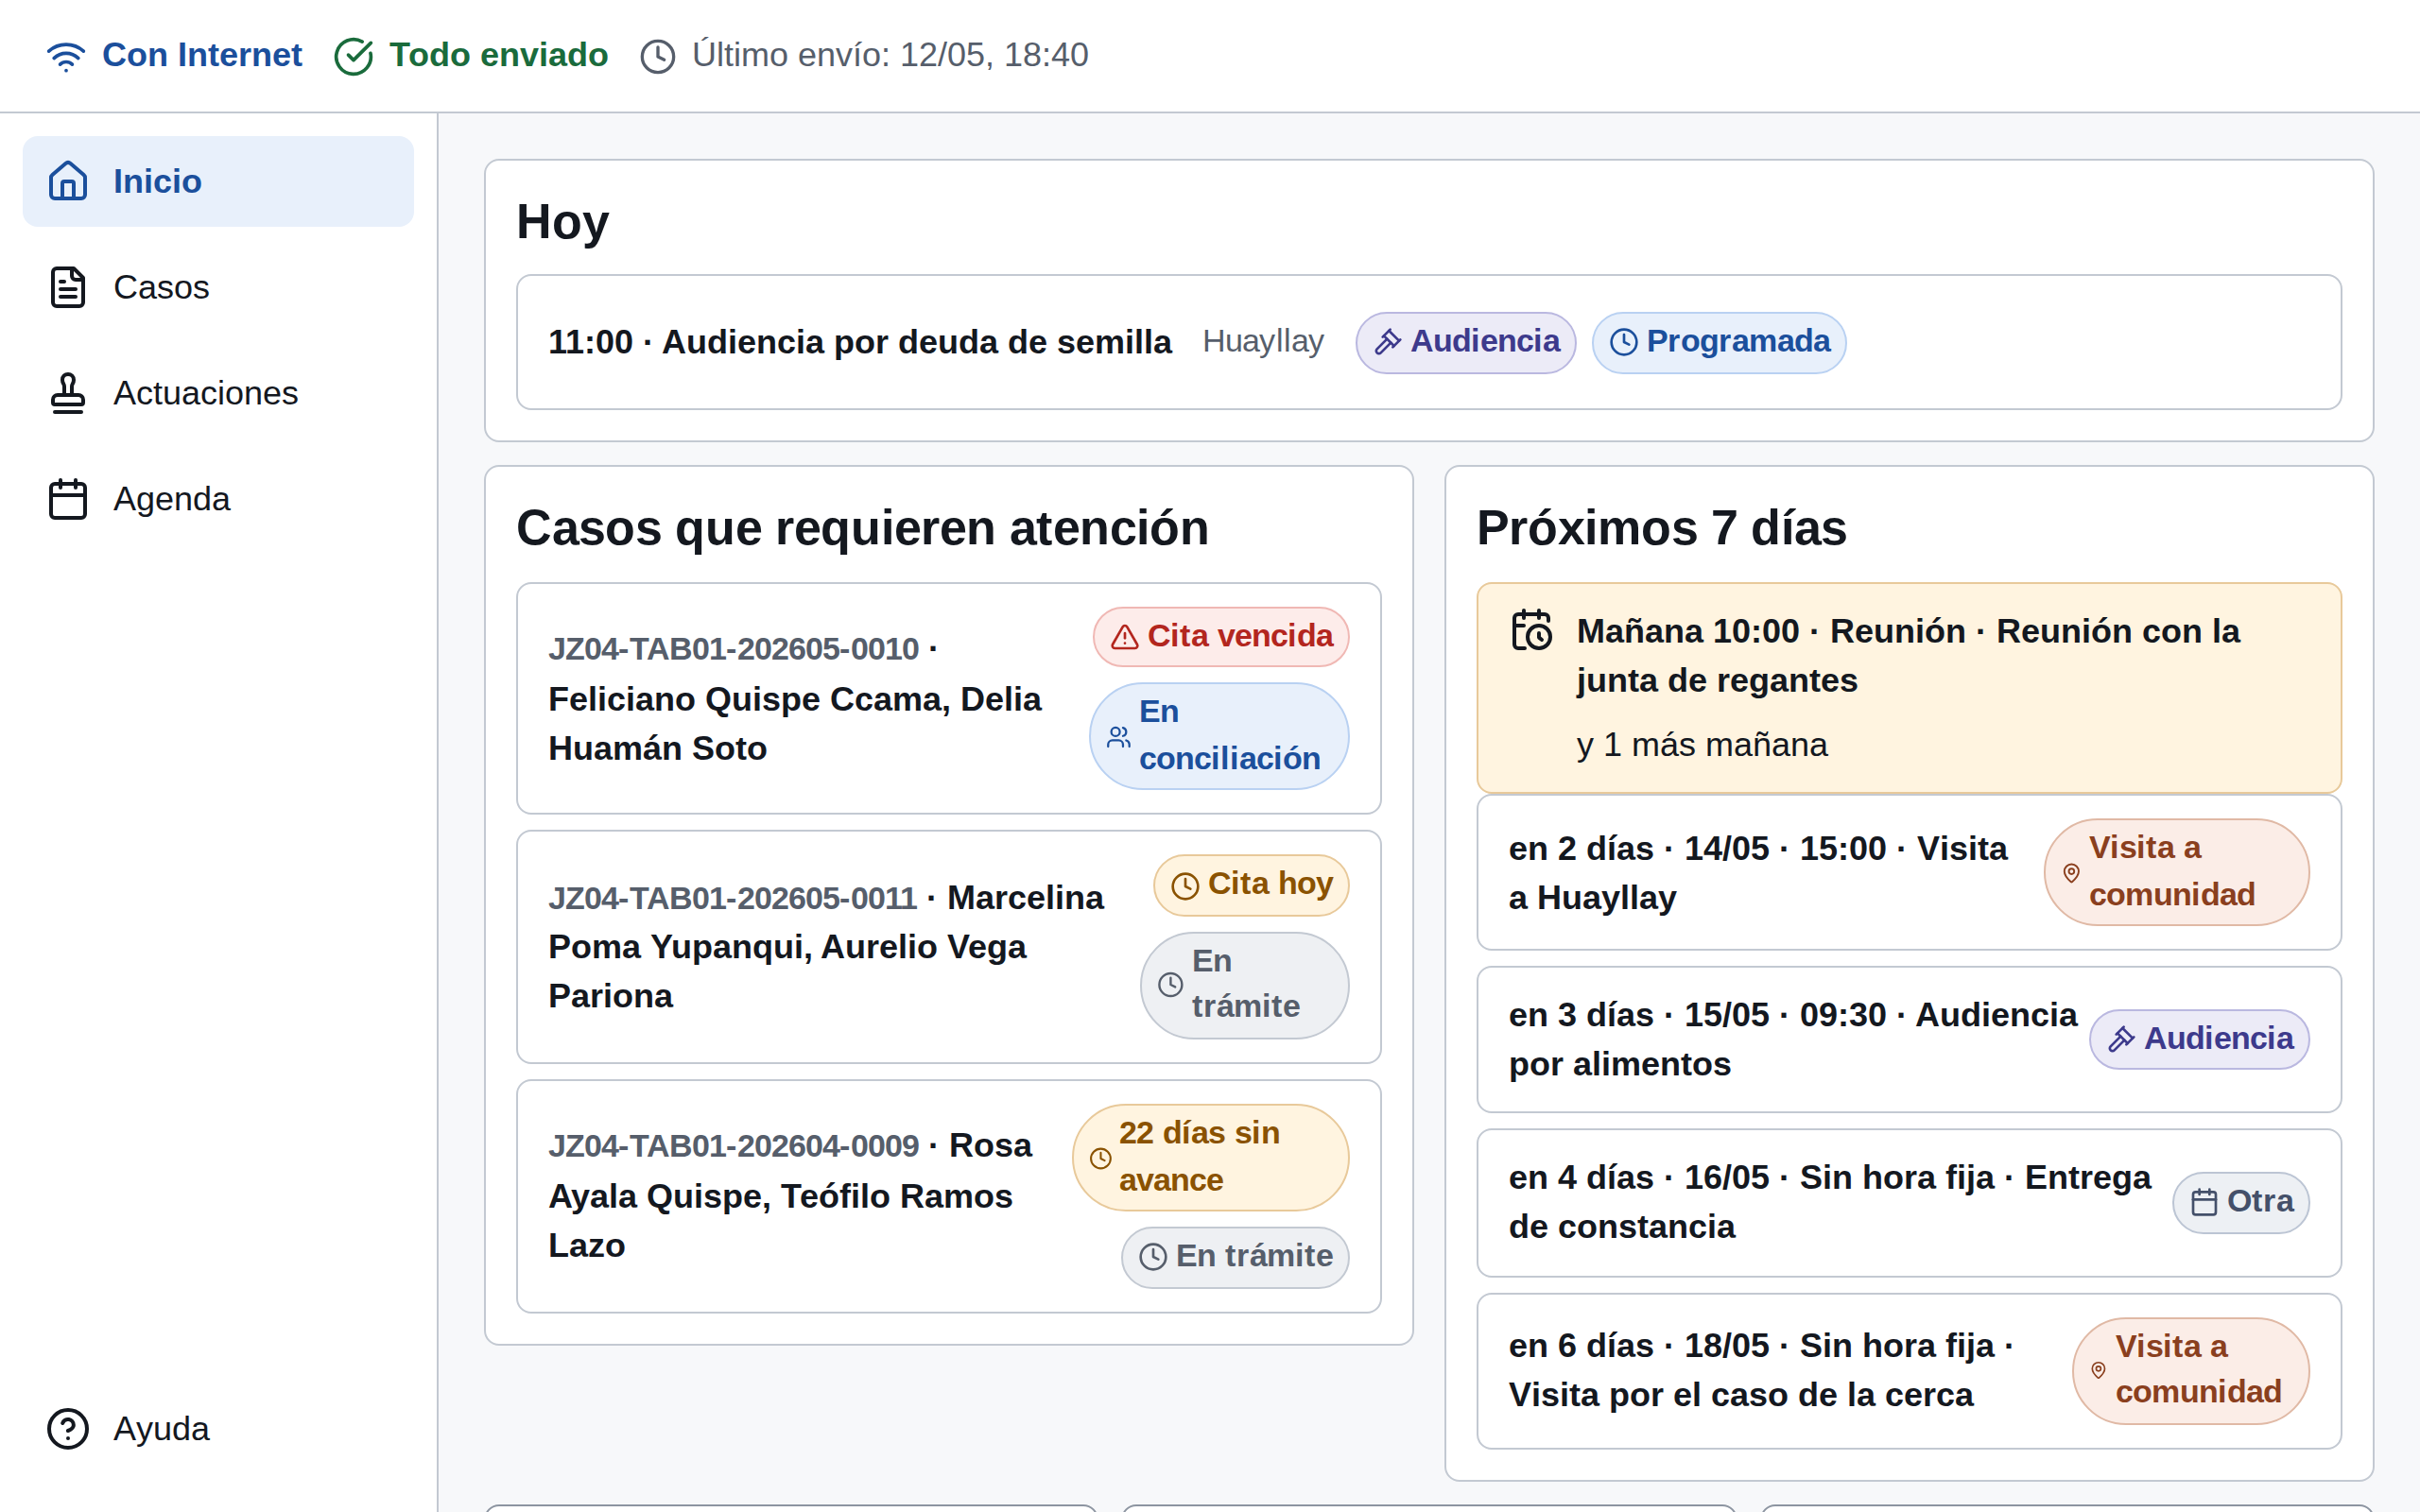
\includegraphics[width=0.86\linewidth]{capturas/P-01_inicio.png}
\caption{P-01 · Estado normal. Inicio con hoy, casos que requieren atención y próximos 7 días}
\end{figure}
\begin{figure}[H]\centering
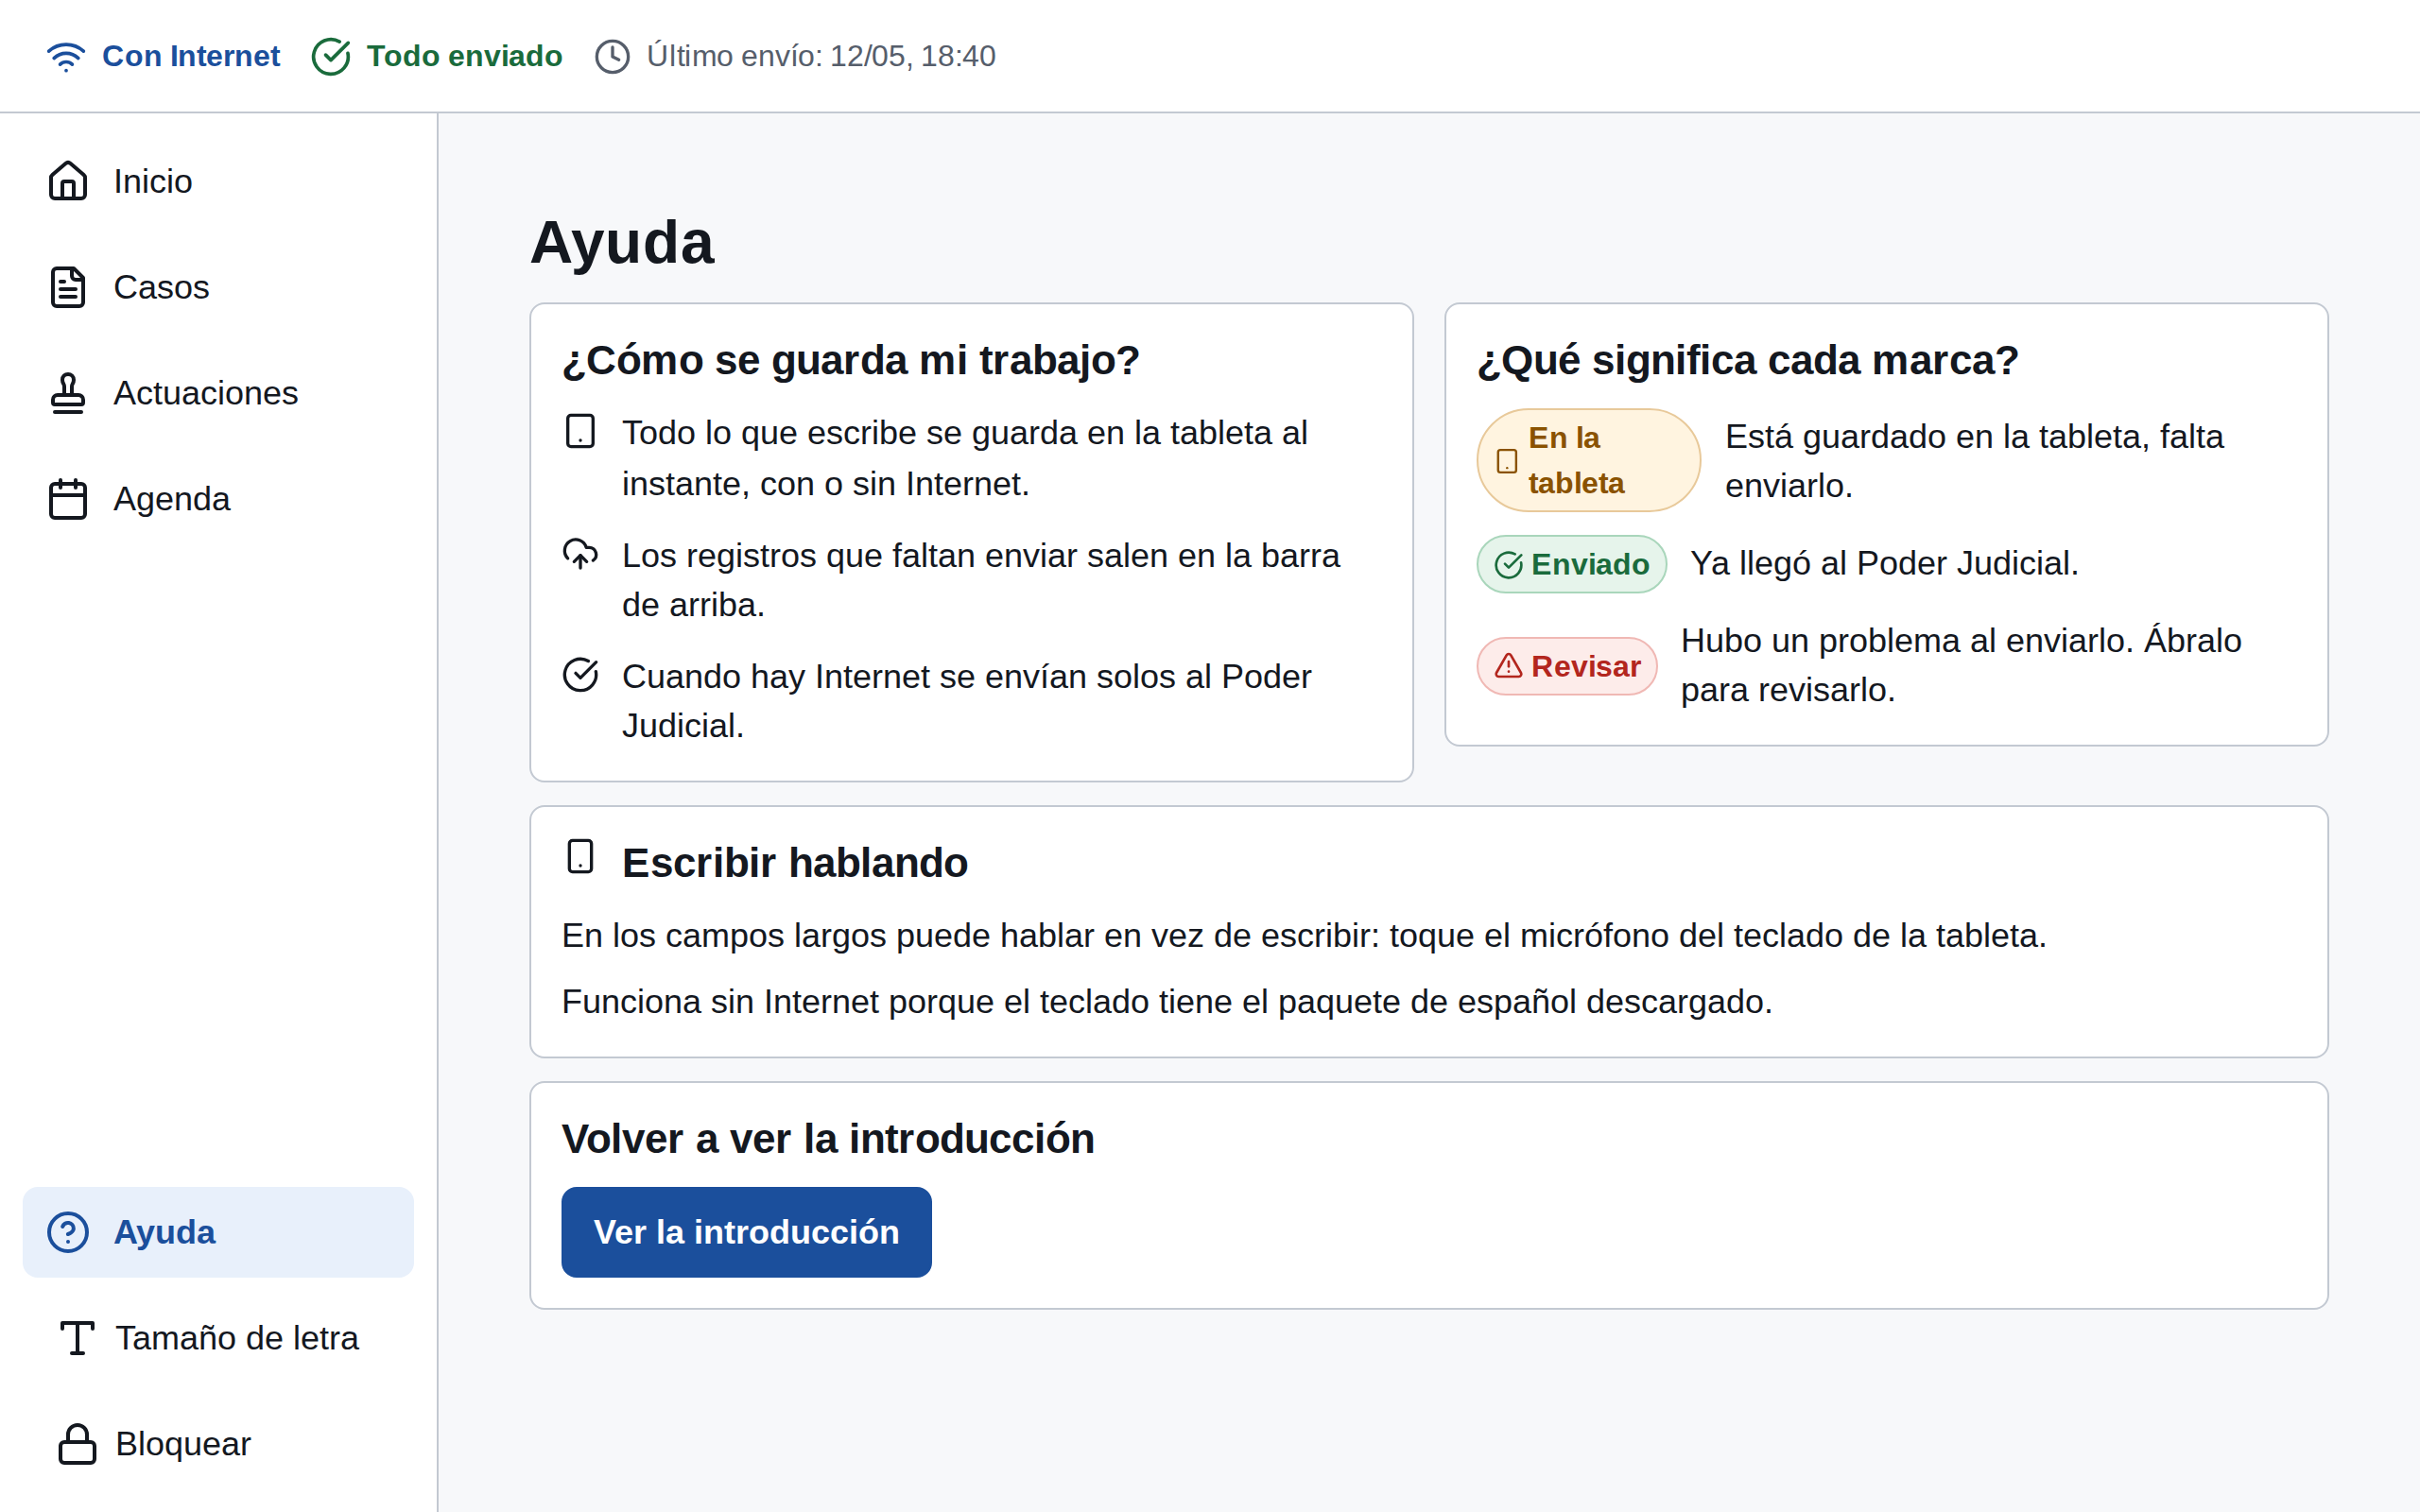
\includegraphics[width=0.86\linewidth]{capturas/Ayuda_ayuda.png}
\caption{Ayuda · Estado normal. Ayuda con el significado de cada marca y el dictado del teclado}
\end{figure}
